\documentclass[fleqn,10pt]{wlscirep}
\title{Assessing heterogeneity (and predictability ??) of runners' performance in Switzerland}

\author[1,*]{Gianrocco Lazzari}
\author[2]{Stefano Savaré}
\author[2]{Antonio Iubatti}
\author[2]{Maxime Peschard}
\author[2]{Ondine Chanon}
\author[3]{Michele Catasta}
\author[1]{Marcel Salathé}

\affil[1]{Global Health Institute, School of Life Sciences, Ecole Polytechnique Fédérale de Lausanne (EPFL), Lausanne, Switzerland.}
\affil[2]{School of Computer Science, Ecole Polytechnique Fédérale de Lausanne (EPFL), Lausanne, Switzerland.}

\affil[3]{Department of Computer Science, Stanford University, Stanford, USA.}


\affil[*]{gianrocco.lazzari@epfl.ch}

%\affil[+]{these authors contributed equally to this work}

%\keywords{Aging, Distance running, Endurance performance, Sex difference}

%%%% %%%% %%%% %%%%  GR's packages %%%% %%%% %%%% %%%% %%%% 

\usepackage{caption,subfigure,float}
%\usepackage{subcaption} 

% for an examples please fer to http://tex.stackexchange.com/questions/148438/putting-two-images-beside-each-other

%packages for references
\usepackage{hyperref,url,cite}


%%%% %%%% %%%% %%%% %%%% %%%% %%%% %%%% %%%% %%%% %%%% %%%% 

\begin{abstract}
	
%Example Abstract. Abstract must be under 200 words and not include subheadings or citations. 



	\textbf{keywords}: Aging, Distance running, Endurance performance, Sex difference

\end{abstract}
\begin{document}

\flushbottom
\maketitle
% * <john.hammersley@gmail.com> 2015-02-09T12:07:31.197Z:
%
%  Click the title above to edit the author information and abstract
%
\thispagestyle{empty}

%\noindent Please note: Abbreviations should be introduced at the first mention in the main text – no abbreviations lists. Suggested structure of main text (not enforced) is provided below.

\section*{Introduction}

%The Introduction section, of referenced text\cite{Figueredo:2009dg} expands on the background of the work (some overlap with the Abstract is acceptable). The introduction should not include subheadings.

as show in \cite{connick2015relative} blabalblab 

\section*{Results}

%Up to three levels of \textbf{subheading} are permitted. Subheadings should not be numbered.
%
%\subsection*{Subsection}
%
%Example text under a subsection. Bulleted lists may be used where appropriate, e.g.
%
%\begin{itemize}
%\item First item
%\item Second item
%\end{itemize}
%
%\subsubsection*{Third-level section}
% 
%Topical subheadings are allowed.

	\subsection*{Demographics}
	
		In fig. \ref{participation_overall_by_distance} and \ref{participation_overall_by_gender} we show respectively how the number of runners increased in the last 15 years, by distances and gender. 
		This raise was steeper for man than for women (fig. \ref{participation_overall_by_gender}), and steeper in the shorter distance (10 Km) than in the longer ones ( fig. \ref{participation_overall_by_distance} - participants in full marathons seems to have decreased though) \footnote{For simplicity we only include the most popular distances. 
		There are many events that include shorter distances, like 3 Km, 5 Km, usually attended by a small fraction of young runners.}.
	
		\begin{figure}[h]	
	
			\centering
			
			\subfigure[]{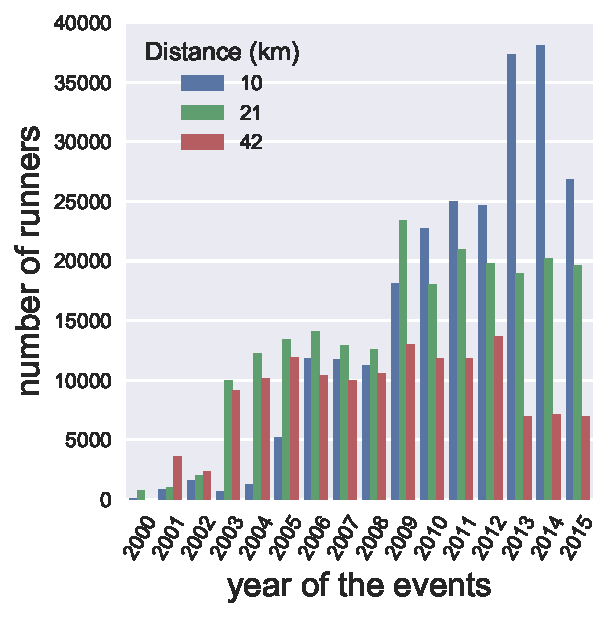
\includegraphics[scale=0.8]{../data_analysis/plots_for_paper/participation_overall_by_distance.pdf}\label{participation_overall_by_distance}}
%					\hfill
			\subfigure[]{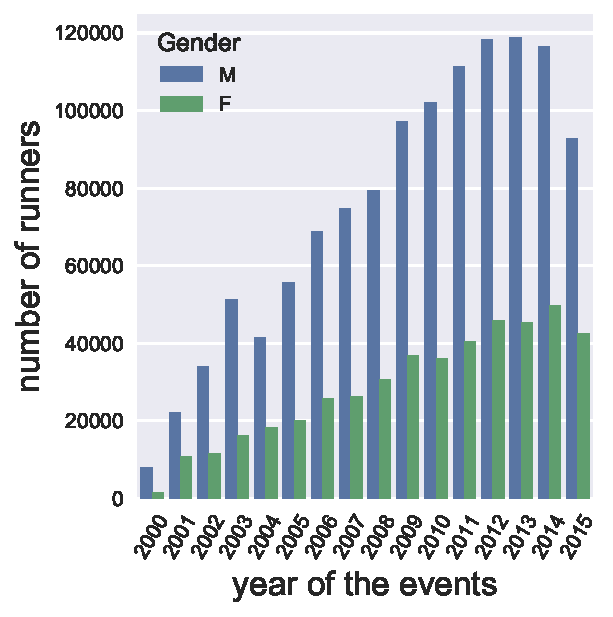
\includegraphics[scale=0.8]{../data_analysis/plots_for_paper/participation_overall_by_gender.pdf}\label{participation_overall_by_gender}}
			
			\caption{Number of participants in running competition in Switzerland, across time, by distance (a) and gender (b).}
		
		\end{figure}		
	
		For a significant analysis of runners' performance, it is important to check the amount of data present in the various events, and therefore first assess the heterogeneity of  events popularity.
		In fig. \ref{dist_number_editions_race} we show the  distribution of number of editions each event was hosted, across all history. Counting all editions of  all races as independent, we recorded 222 events. 
		More interestingly in fig. \ref{number_runners_per_race} one can see the broad distribution of number of participants in the different events. In particular, a power-law fit  ( $ f(x) \sim x^{-\alpha} $) provides an exponent of $ \alpha = 1.69 \pm 0.05 $\footnote{The power-law starts from  a lower-bound, whose value results as well from the fitting procedure: $ x_{min} = 688  $ runners/race}.
		
		\begin{figure}[h]	
			\centering
			
			\subfigure[]{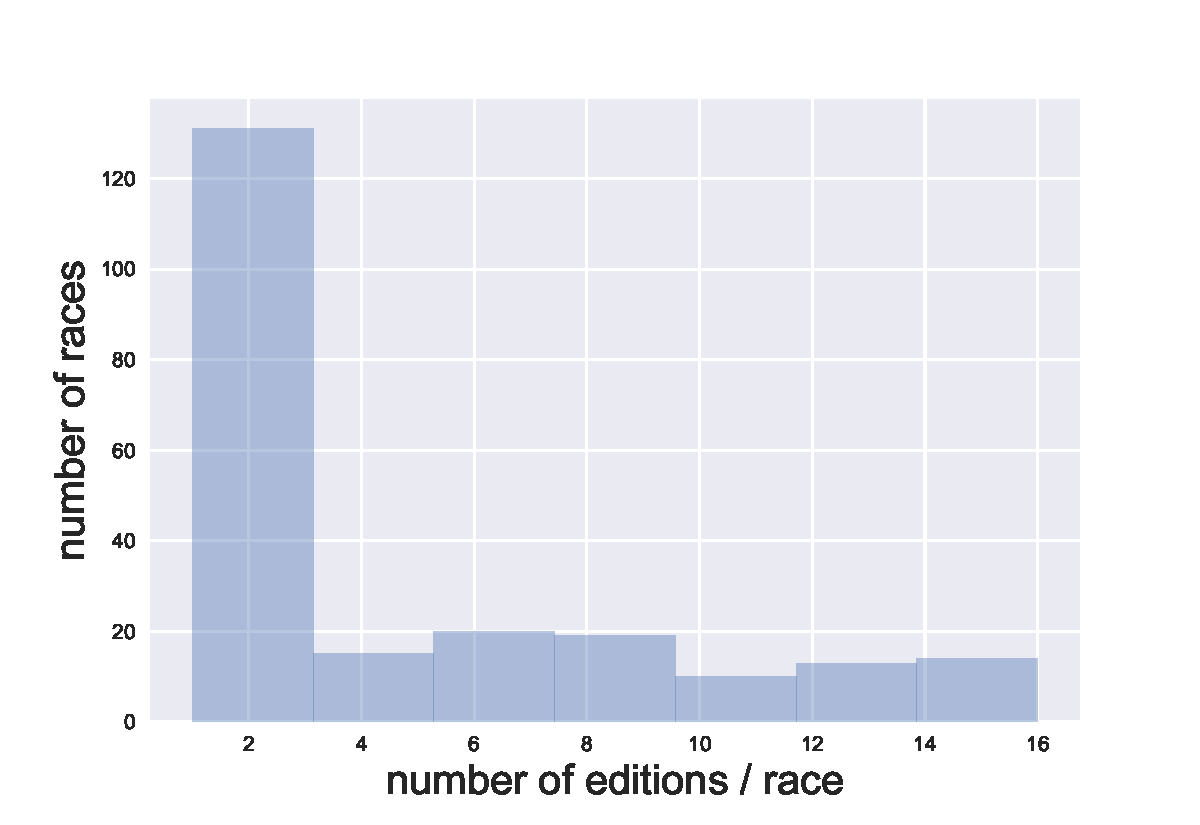
\includegraphics[scale=0.4]{../data_analysis/plots_for_paper/dist_number_editions_race.pdf}\label{dist_number_editions_race}}
			%					\hfill
			\subfigure[]{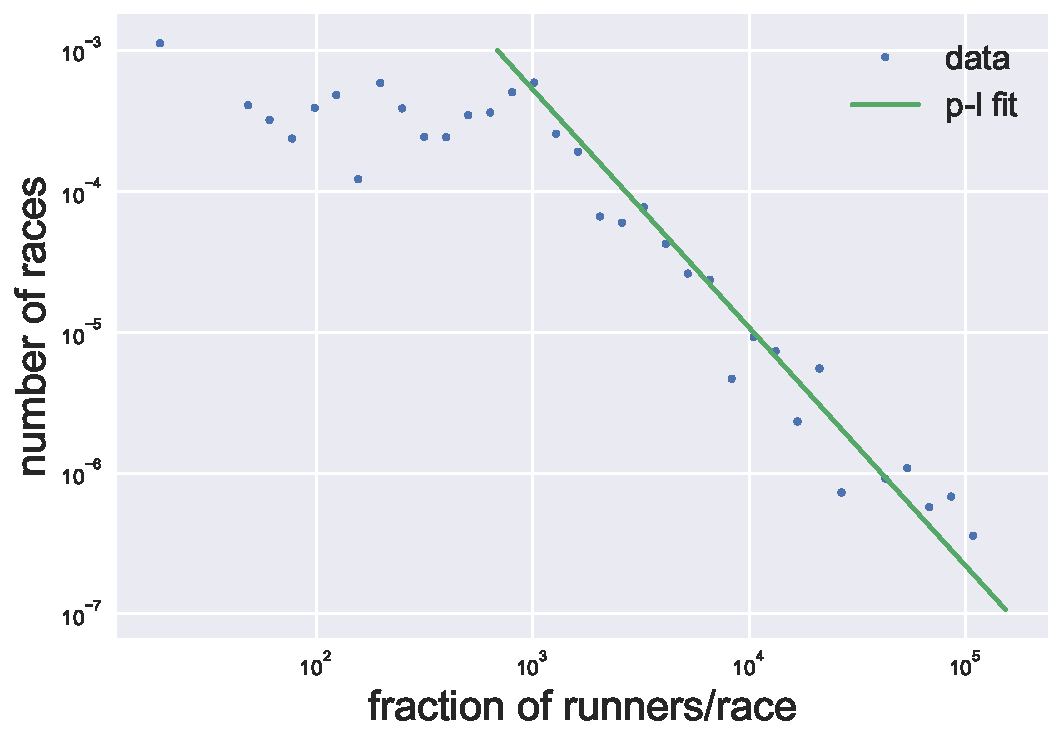
\includegraphics[scale=0.4]{../data_analysis/plots_for_paper/number_runners_per_race.pdf}\label{number_runners_per_race}}
			
			\caption{Assess popularity of running competitions, in Switzerland.}
		\end{figure}		
	
		Inversely, one can measure how participative runners have been across Switzerland. 
		In fig. \ref{number_races_per_runner} we show the distribution\footnote{		One can see that a log-normal would fit better in this case than a power-law model. In particular the fitted parameters are $ \mu = -0.70, \sigma  = 1.55 $} of  the number of events to which each runners participated. We collected data from  a total number of 531426 runners.

		
		
		\begin{figure}[h]	
			\centering
			
			\subfigure[]{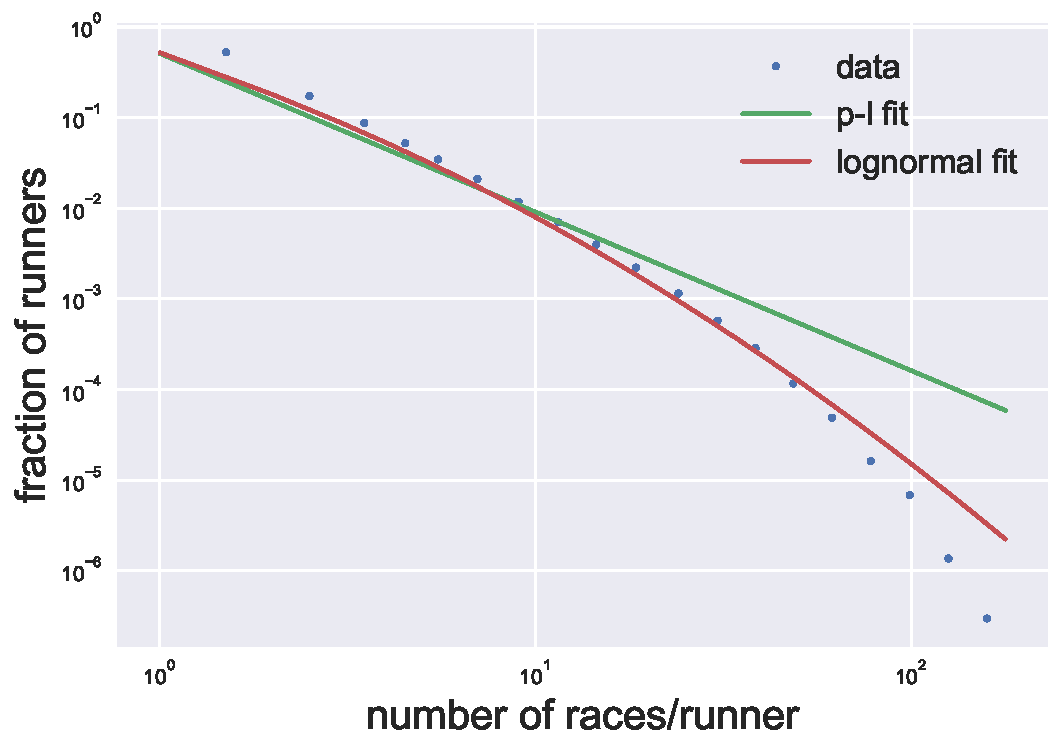
\includegraphics[scale=0.4]{../data_analysis/plots_for_paper/number_races_per_runner.pdf}\label{number_races_per_runner}}
			%					\hfill
%			\subfigure[]{\includegraphics[scale=0.4]{../data_analysis/plots_for_paper/}\label{}}
			
			\caption{Assess how participative runners are across competitions, in Switzerland.}
		\end{figure}					
			
	\subsection*{The case of Lausanne Marathon}
		
		We consider the case of 2016 Lausanne Marathon event to present some relevant statistics on age and performance distribution, due to his popularity across all Switzerland (see indeed also fig. \ref{origin_towns_dist} for the distribution of runners' origin towns).
		Apart from the 812 kids (younger than 14 years) running  a shorter race, the 2016 edition had over 10K participants, divided per race  and gender, as shown in table \ref{counts_per_distance} (\textbf{set the 2 tables next to each other!})


% thanks to http://truben.no/table/

	 	\begin{table}
	 		\begin{tabular}{l|l}
	 			Category     & Number of participants \\ \hline
	 			10 km         & 5515                   \\
	 			half-marathon & 4414                   \\
	 			marathon      & 1318                   \\
	 		\end{tabular}
 		
 			\begin{tabular}{l|l}
				Gender     		& Number of participants \\ \hline
 				M       	  & 6905 					\\
				F		 		& 4655                   \\
 			\end{tabular}
 		\caption{Number of participants in 2016 Lausanne Marathon}
 		\label{counts_per_distance}
	 	\end{table}
 	
 		In fig. \ref{women_age_dist_lausanne} and \ref{men_age_dist_lausanne}
 		
 		
		\begin{figure}[h]	
			\centering
			
			\subfigure[]{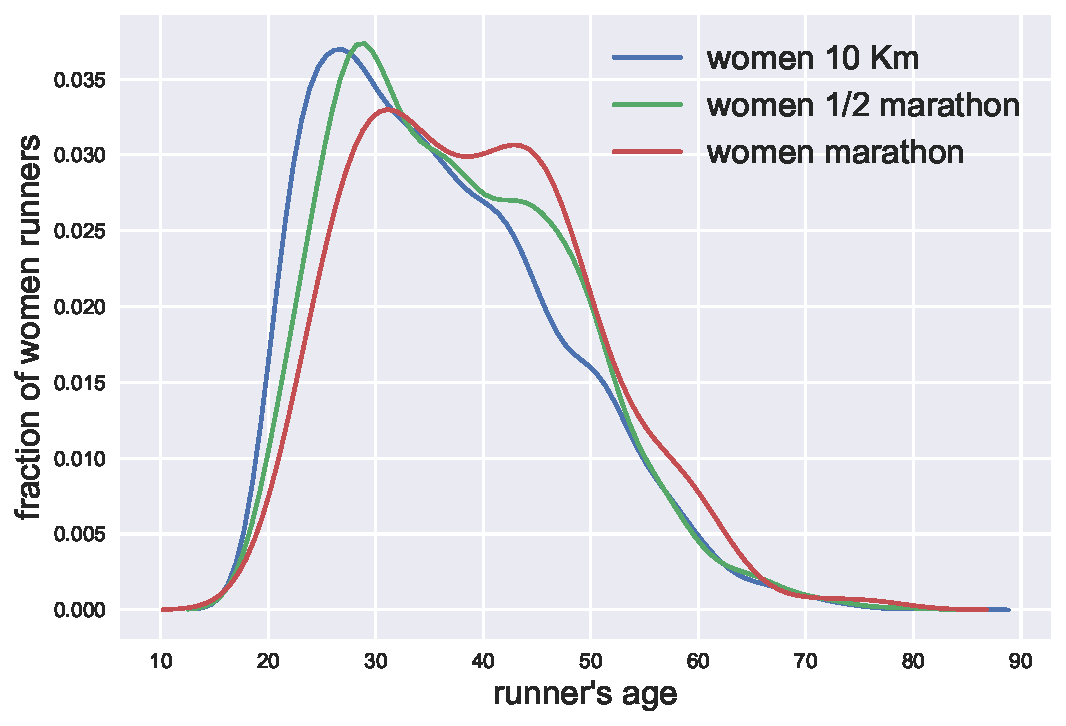
\includegraphics[scale=0.4]{../data_analysis/plots_for_paper/women_age_dist_lausanne.pdf}\label{women_age_dist_lausanne}}
			%					\hfill
			\subfigure[]{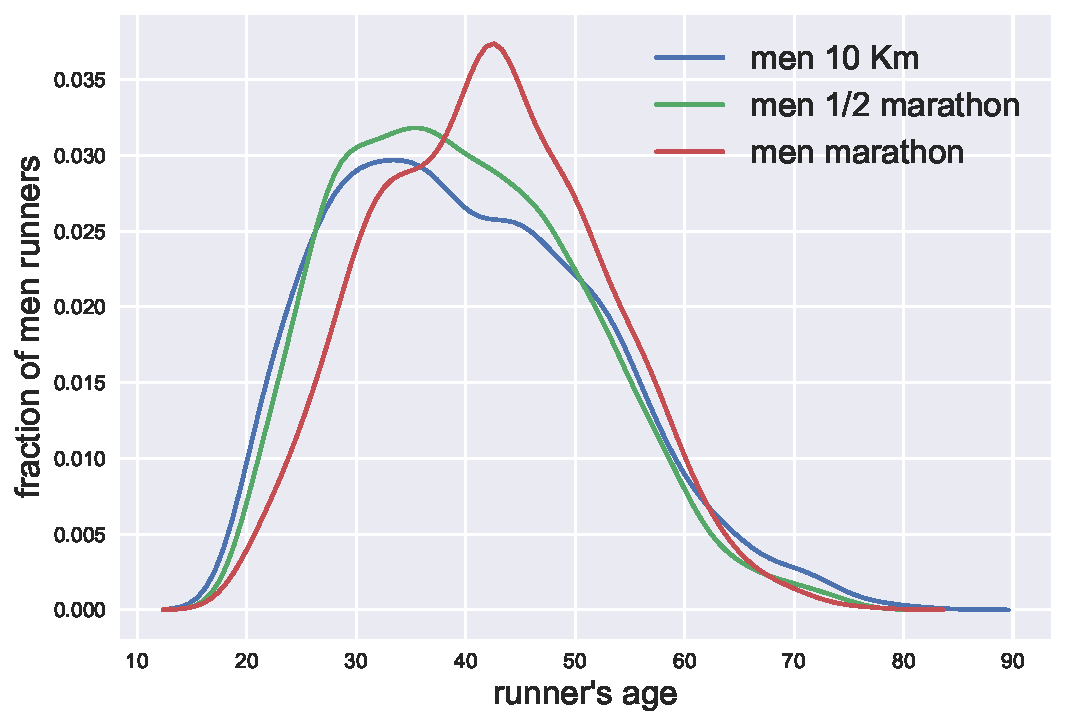
\includegraphics[scale=0.4]{../data_analysis/plots_for_paper/men_age_dist_lausanne.pdf}\label{men_age_dist_lausanne}}
			
			\caption{Runners' age distribution in 2016 Lausanne Marathon, for women (a) and men (b) and divided by race (color-coded).}
		\end{figure}		 		
		 		
	
	
	\subsection*{Overall performance analysis}
	
		\subsubsection*{Age-performance relation}
		
		
			We wanted to check whether the previously found	\cite{connick2015relative,knechtle2014relationship,lara2014relationship,lehto2016effects}
			U-relation between age and performance holds as well in the case of swiss races. 
			In fig. \ref{performance_VS_age_marathon} 
			(\textbf{plot to be improved!}) 
			we show the dependence of runners' performance on age, for four of the most popular swiss marathons. 
			The above-mentioned U-shaped although still slightly appearing in the longest distance (42Km), it does emerge more clearly in the half-marathons, as  shown indeed in fig. \ref{performance_VS_age_semi_marathon}
			(\textbf{plot to be improved!}) 
			
			
			\begin{figure}[h]	
		
				\centering
				
				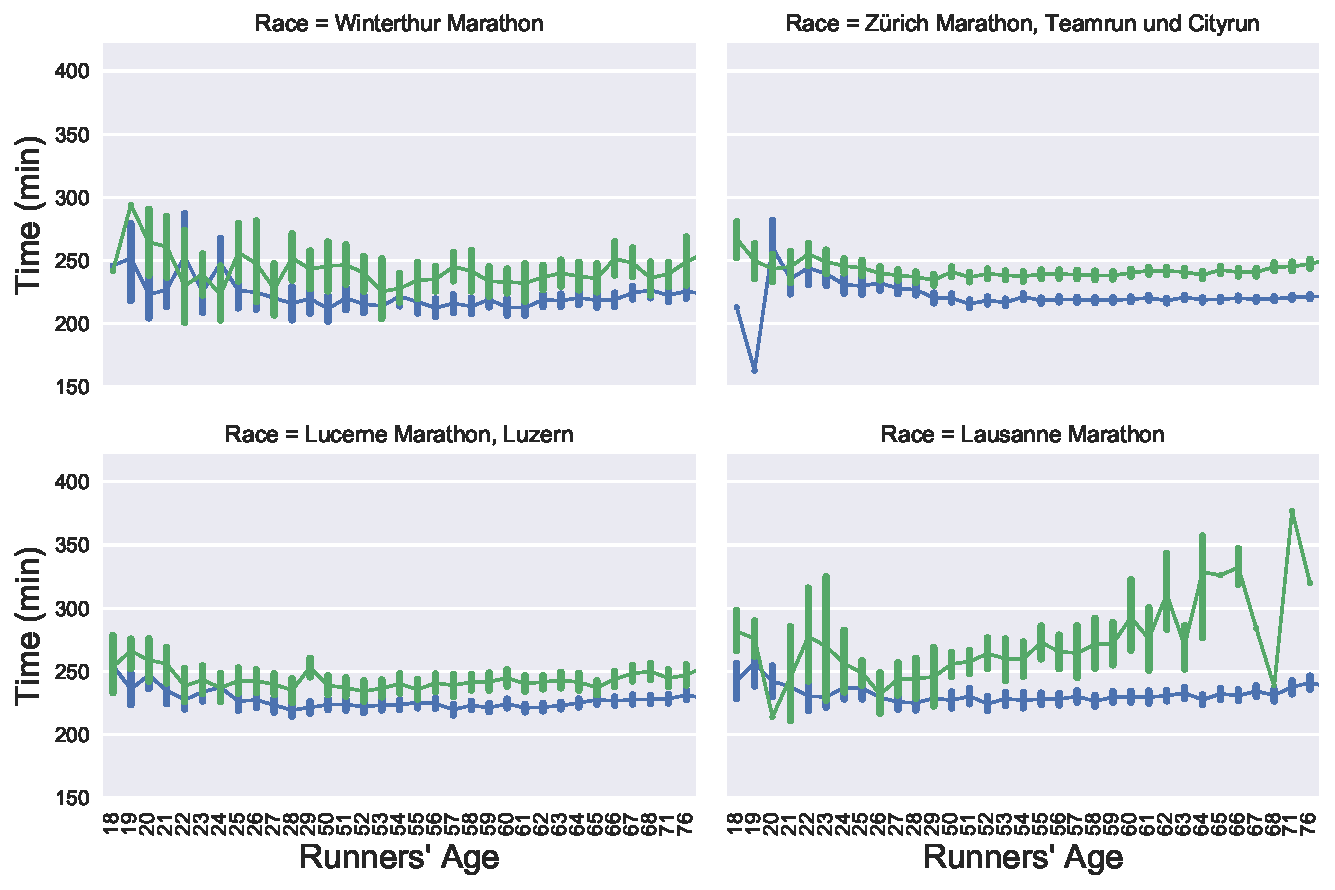
\includegraphics[scale=0.6]{../data_analysis/plots_for_paper/performance_VS_age_marathon.pdf}
				
				%				\subfigure[]{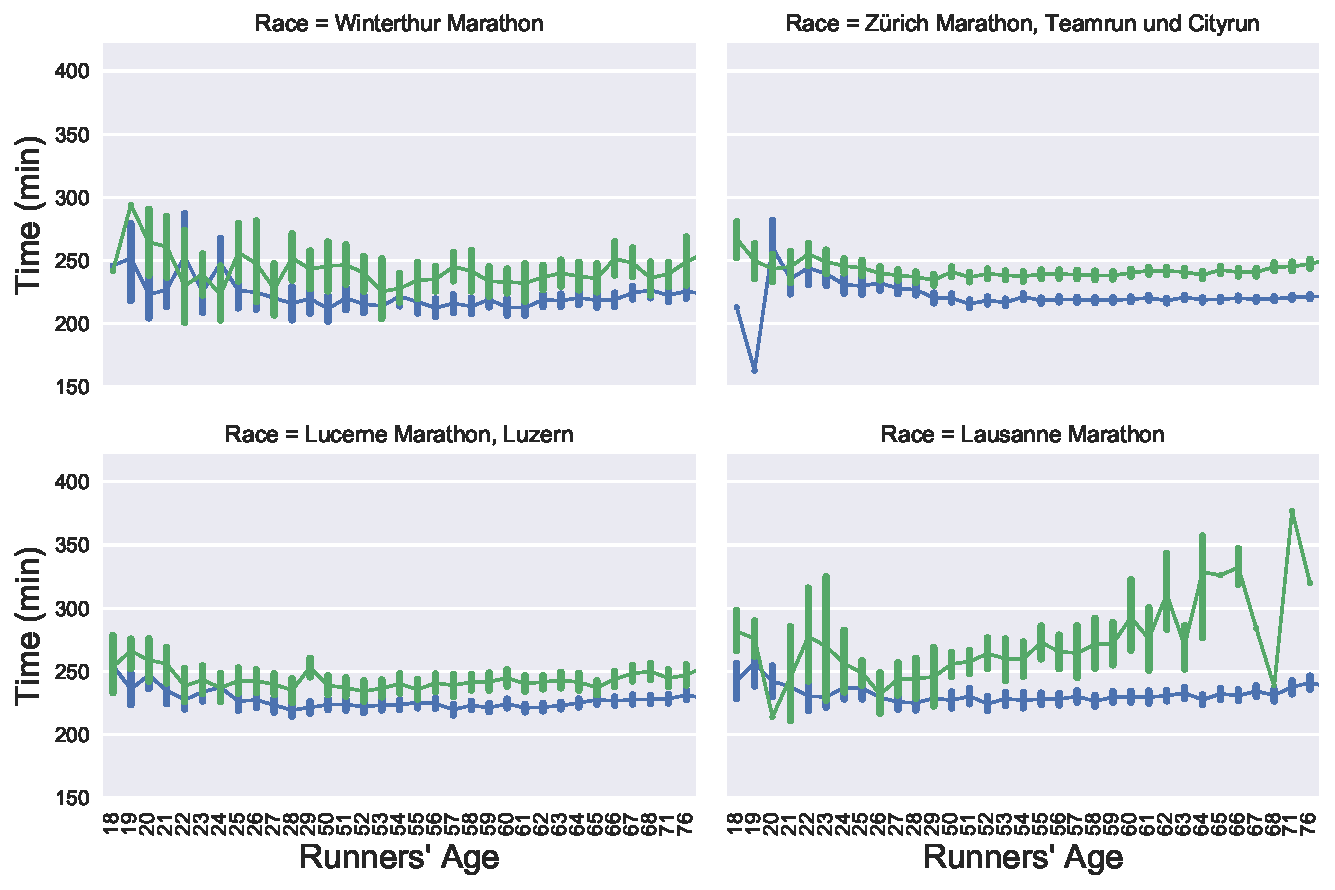
\includegraphics[scale=0.35]{../data_analysis/plots_for_paper/performance_VS_age_marathon.pdf}\label{performance_VS_age_marathon}}
				%					\hfill
				%						\subfigure[]{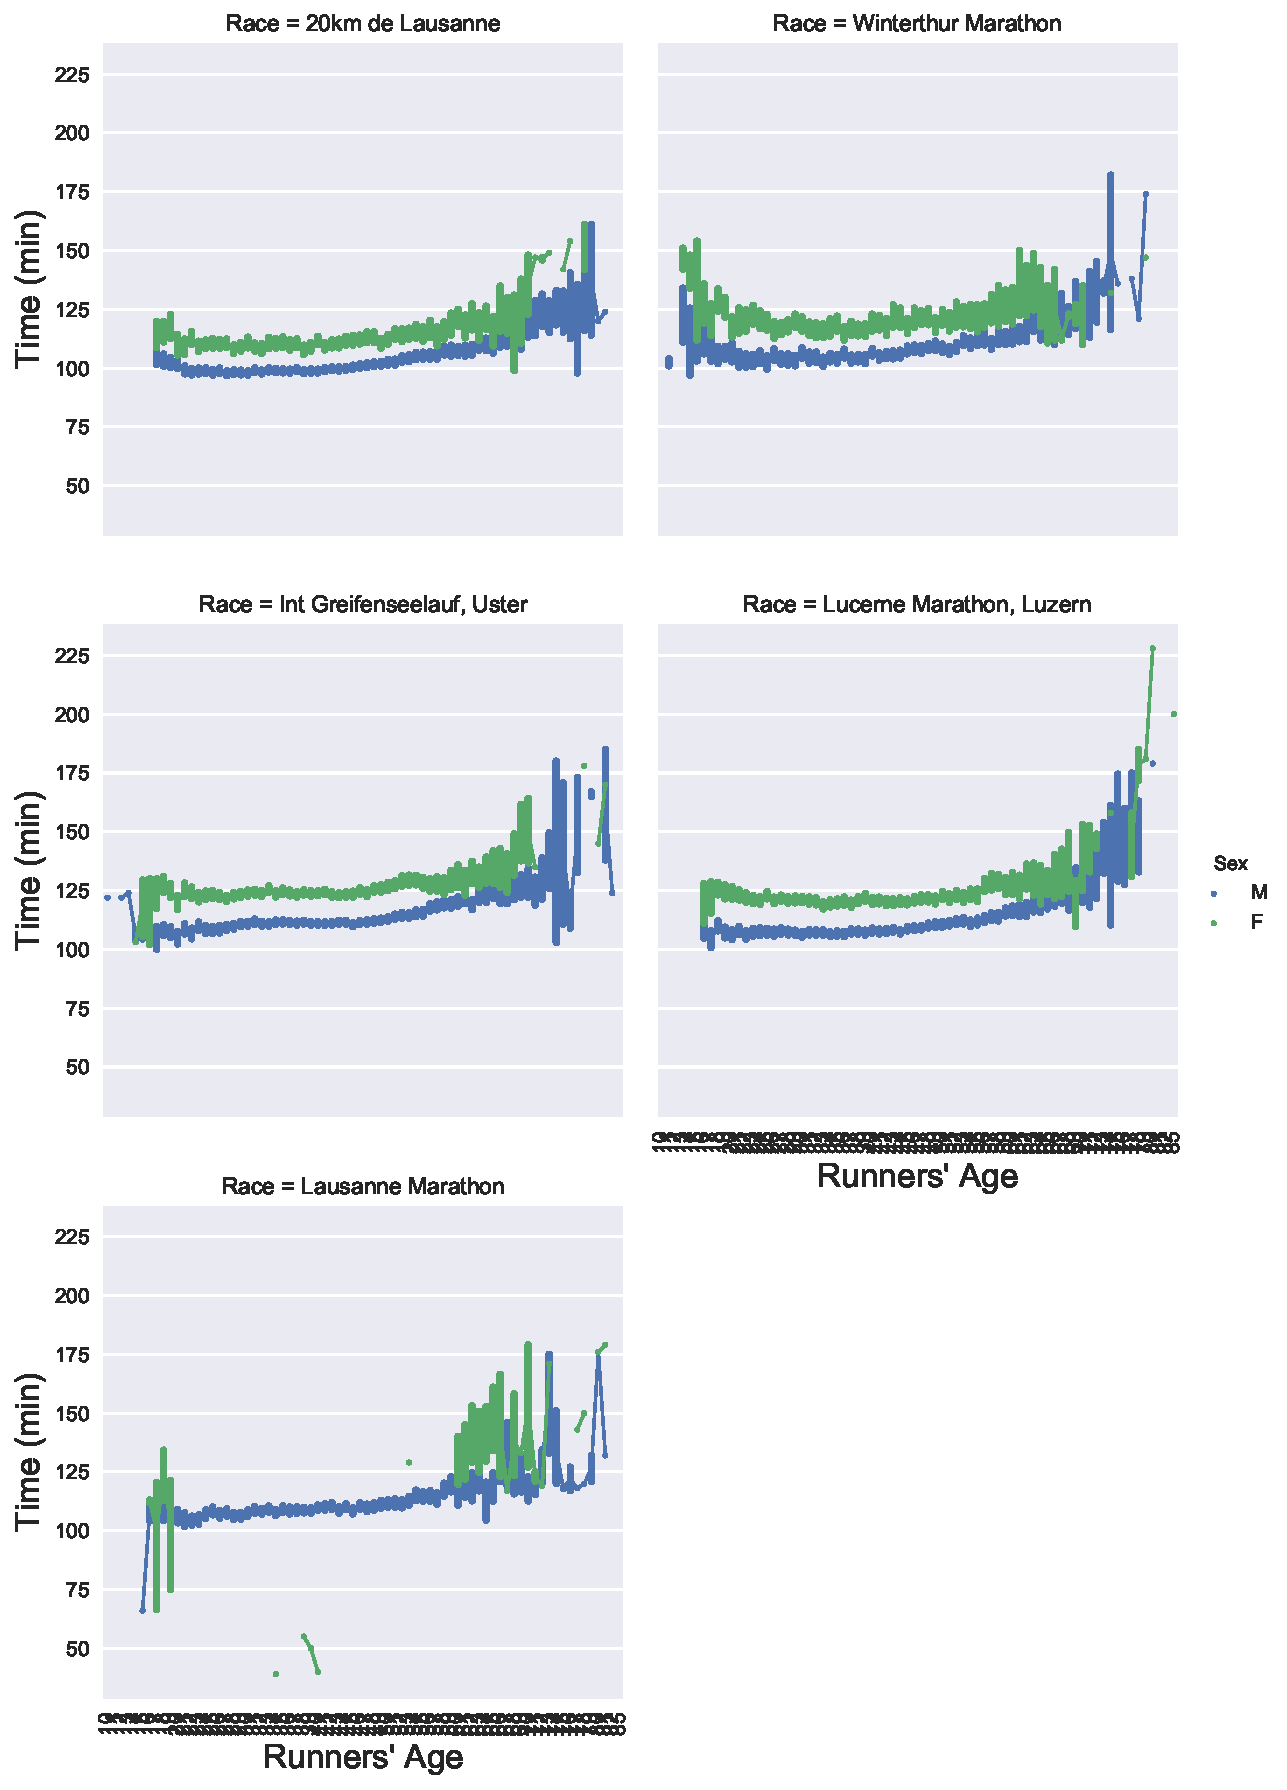
\includegraphics[scale=0.35]{../data_analysis/plots_for_paper/performance_VS_age_semi_marathon.pdf}\label{performance_VS_age_semi_marathon}}
				
				\caption{Relation between runners' performance (time in minutes to complete the race) and age, for the most popular marathons, color coded by gender.}
				
				\label{performance_VS_age_marathon}
		
			\end{figure}								
		
		
			\begin{figure}[h]	
			
				\centering
				
				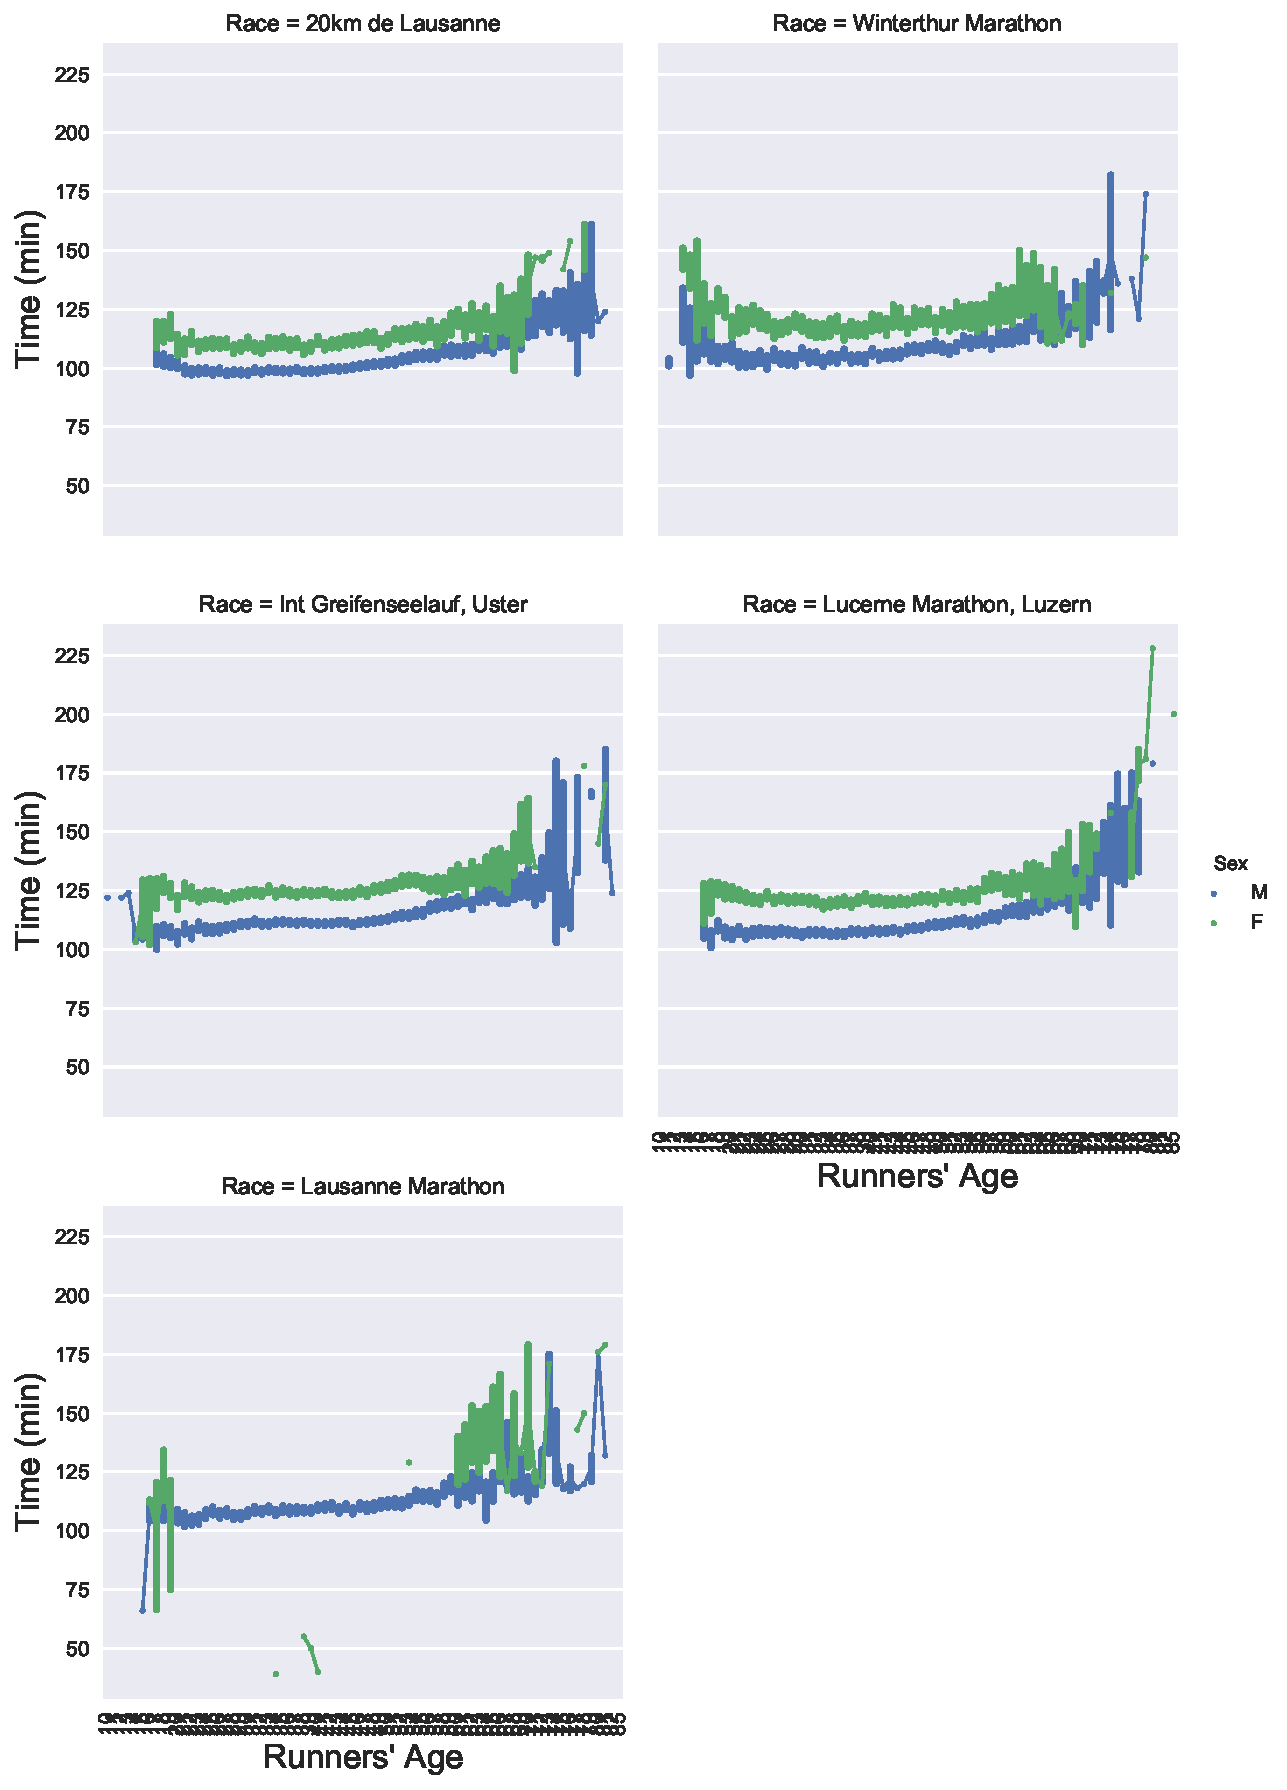
\includegraphics[scale=0.6]{../data_analysis/plots_for_paper/performance_VS_age_semi_marathon.pdf}
				
				\caption{Relation between runners' performance (time in minutes to complete the race) and age, for the most popular half-marathons (20 Km and 21 Km), color coded by gender.}
				
				\label{performance_VS_age_semi_marathon}
			
			\end{figure}								
			
		\subsubsection*{Temperature-performance relation}
		
			we don't have enough data (can be re-checked)...\\
			
			some reviews on the topic:\\
			\url{http://runningstrong.com/temperature.html}\\
			\url{http://believeperform.com/performance/the-effects-of-heat-on-sport-performance/}
			
	
	
		\subsection*{Geographical analysis}
	
			(to be included ??)(by Antonio \& Gr) \\			
			
			It is interesting to assess from which cities runners come, and how many of them, from the different locations. 
			In fig. \ref{origin_towns_dist} we report as an example the quite 
			broad\footnote{Fittetd exponent: $ \alpha = 1.90 \pm 0.03 $} distribution of number of runners, coming from the 2005 municipalities reported for the 2016 Lausanne Marathon.
			
			\begin{figure}[h]	
				
				\centering
				
				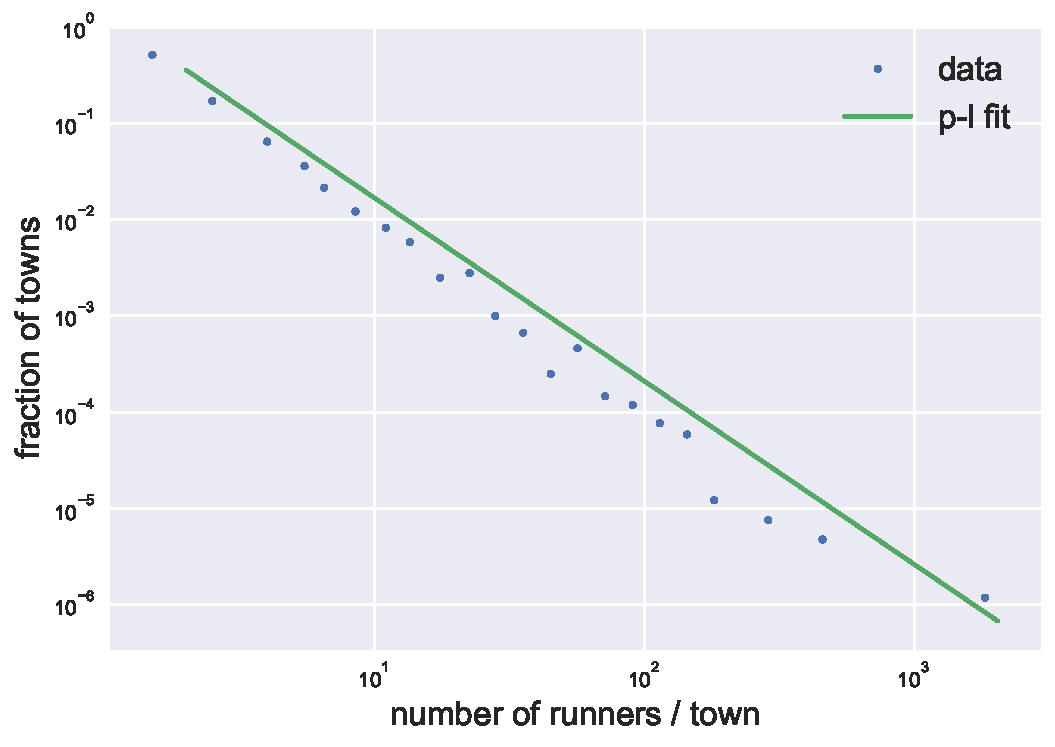
\includegraphics[scale=0.6]{../data_analysis/plots_for_paper/origin_towns_dist.pdf}
				
				\caption{}
				
				\label{origin_towns_dist}
				
			\end{figure}								
	
		\subsection*{Network of runners}
	
				(to be included ??)
				(by Gr)
		
		\subsection*{Forecast of career advancement (??)}
	
				(not done yet)		\\
				\href{https://fivethirtyeight.com/features/tell-us-two-things-and-well-tell-you-how-fast-youd-run-a-marathon/}{nice article on fivethertyeight},
				pointing to one of the best/latest model \cite{vickers2016empirical}

	

\section*{Discussion}

%The Discussion should be succinct and must not contain subheadings.

\section*{Methods}

%Topical subheadings are allowed. Authors must ensure that their Methods section includes adequate experimental and characterization data necessary for others in the field to reproduce their work.

	\subsection*{Data parsing}
	
		@stefano 
		(remember to add the \textit{definition of runner})
	
		
	
	
	\subsection*{Data analysis}
	
		All analysis were performed on python notebooks (available on the \href{related repository}{related repository}), using standard python packages for data analysis and plotting, such as \texttt{pandas}, \texttt{seaborn}, \texttt{scipy}, \texttt{powerlaw}\footnote{\url{https://pypi.python.org/pypi/powerlaw}} and \texttt{networkx}.
	
	
	\subsection*{Data visualization}		
	
		We implemented interactive visualizations of some of our results and collected  them in the   \href{https://hopsuisse.github.io}{Hop Suisse}\footnote{\url{https://hopsuisse.github.io}} website.
		After exporting the data needed for the plot in \texttt{.json} dumps, we used \href{http://c3js.org}{C3.js} for the interactive plotting. More details on how datasets queries and plots were built can be found on the dedicated \href{https://github.com/hopsuisse/hopsuisse.github.io}{GitHub repository}\footnote{\url{https://github.com/hopsuisse/hopsuisse.github.io}}.
		We also build an \href{https://www.youtube.com/watch?v=MyvbnOXHShw}{animated infographics}\footnote{\url{https://www.youtube.com/watch?v=MyvbnOXHShw}}, inspired by  \href{https://en.wikipedia.org/wiki/Hans_Rosling}{Hans Rosling}'s work. With such video we wanted to show in a more powerful and clear way the relations among runners' mean pace, experience and age, providing as well information on gender and race length
		(the python code used to construct the video frames can be found in the \href{https://github.com/ggrrll/hop_suisse_ada_project_public/tree/master/8-video}{related folder}\footnote{\url{https://github.com/ggrrll/hop_suisse_ada_project_public/tree/master/8-video}} of our GitHub repository).
	

%\section*{Acknowledgements (not compulsory)}
%
%Acknowledgements should be brief, and should not include thanks to anonymous referees and editors, or effusive comments. Grant or contribution numbers may be acknowledged.

\section*{Author contributions statement}

G.L. and A.I. performed the data analysis.
S.S., O.C. and M.P. performed the data parsing.
G.L. and S.S. wrote the manuscript.
M.C. and M.S. review the manuscript.
%M.C. supervised the study.

\section*{Additional information}

All the code used to parse the data from \url{https://www.datasport.com/en/}, for data analysis and visualization can be found in our open GitHub repository: \url{https://github.com/ggrrll/hop_suisse_ada_project_public}.\\

\section*{Competing financial interests}

The authors declare no conflict of interests.


%%%%%% %%%%%% %%%%%% %%%%%%  BIBLIOGRAPHY %%%%%% %%%%%% %%%%%% %%%%%% %%%%%% 

\newpage
\bibliography{bib_hop_suisse}

%\noindent LaTeX formats citations and references automatically using the bibliography records in your .bib file, which you can edit via the project menu. Use the cite command for an inline citation, e.g.  \cite{Figueredo:2009dg}.


%To include, in this order: 
%\textbf{Accession codes} (where applicable); 
%\textbf{Competing financial interests} (mandatory statement). 
%
%The corresponding author is responsible for submitting a \href{http://www.nature.com/srep/policies/index.html#competing}{competing financial interests statement} on behalf of all authors of the paper. This statement must be included in the submitted article file.

%\begin{figure}[ht]
%\centering
%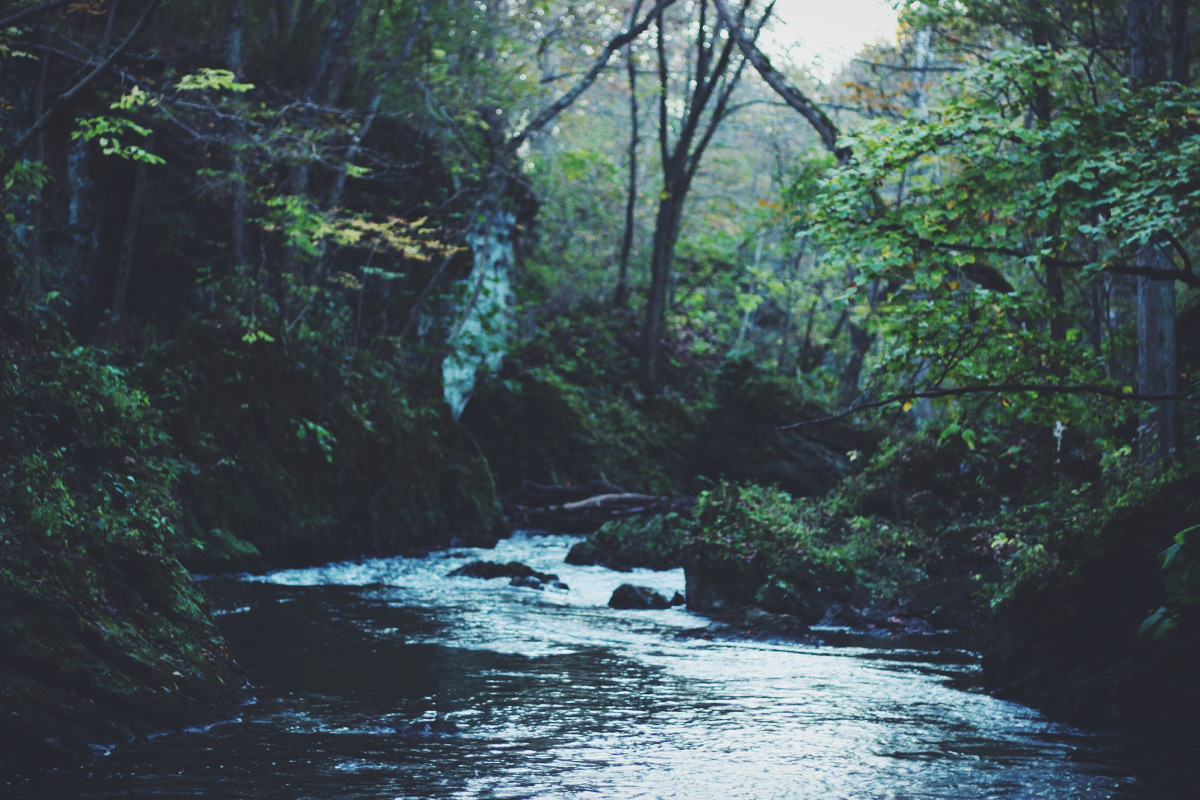
\includegraphics[width=\linewidth]{stream}
%\caption{Legend (350 words max). Example legend text.}
%\label{fig:stream}
%\end{figure}
%
%\begin{table}[ht]
%\centering
%\begin{tabular}{|l|l|l|}
%\hline
%Condition & n & p \\
%\hline
%A & 5 & 0.1 \\
%\hline
%B & 10 & 0.01 \\
%\hline
%\end{tabular}
%\caption{\label{tab:example}Legend (350 words max). Example legend text.}
%\end{table}

%Figures and tables can be referenced in LaTeX using the ref command, e.g. Figure \ref{fig:stream} and Table \ref{tab:example}.

\end{document}